\chapter{Disciplines}
\label{ch:disciplines}

\section{Introduction}
Disciplines provide a wide variety of different extraordinary and/or supernatural options to embelish your campaigns. You can pick and choose what disciplines make more sense to your campaign or you can even come up with your own.

Common in all disciplines is their dependence on certain characteristics. Most use POW and spend Power Points one way or another.

\section{Power}

\subsection{Regaining Power Points}
Using Power Points is a draining and exhausting activity that requires a major effort from which the body needs to recover. Power Points regenerate once the character fully rests, either by sitting down and taking it very easy or by having a good nights sleep. 

For every two hour period that a character rests they regain Power Points equal to a quarter of their POW total.  

\vspace{1em}

\begin{rpg-examplebox}
Rurik, with a POW of 8, takes two hours of rest to regain two Power Points, four hours to regain four Power Points, six hours to regain six Power Points and eight hours to regain the full eight Power Points. 
\end{rpg-examplebox}

\vspace{1em}

Basically, if the character has a comfortable uninterrupted sleep of eight hours they will regain their full power points. Characters may never exceed their original Power Point total by resting.

\vspace{1em}

\subsection{Zero Power Points}
A character who is reduced to zero Power Points falls unconscious until he has regained one Power Point.

\vspace{1em}

\begin{figure}[h]
\begin{center}
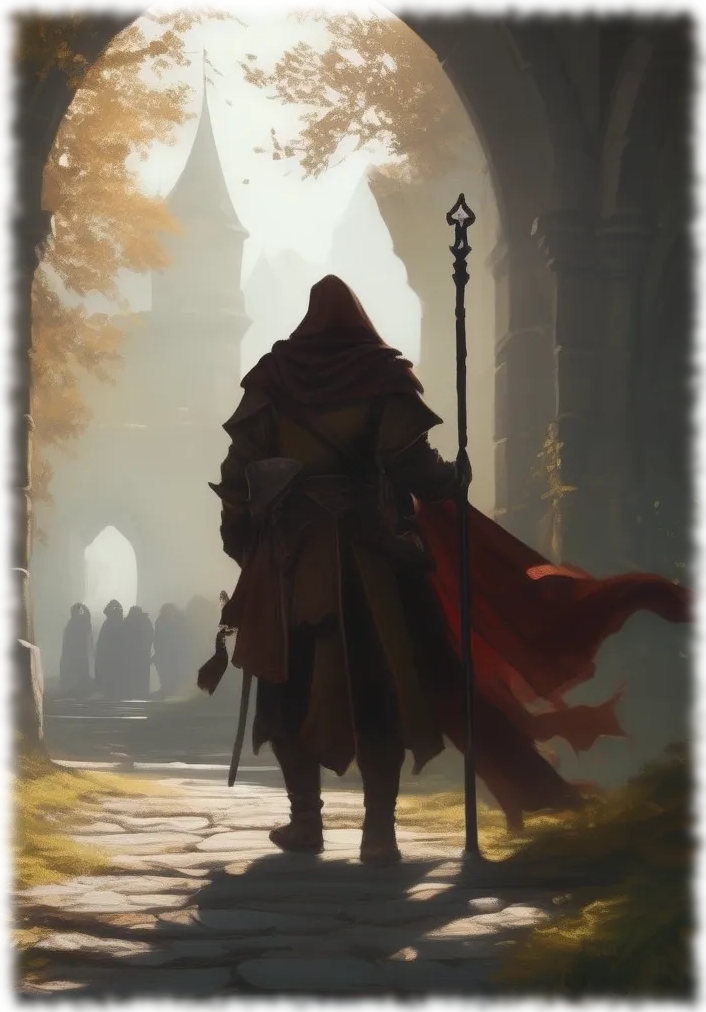
\includegraphics[scale=0.34]{img/ai-images/wizard-from-behind.png}
\end{center}
\end{figure}

\subsection{Beyond Maximum}
There are ways of surpassing the maximum number of Power Points available to characters by using some of the supernatural powers described in the disciplines found in the following chapters. For example, practitioners of the Folk Magic discipline can have access to additional pools of Power Points, via bound Magic Spirits (see Call Spirit spell) and magic items that act as Power Point Stores (see Create Power Point Store spell). However, these pools regenerate, if at all, independently of the character’s natural rate. Experienced Folk Magic users could potentially have several Power Point stores and bound Magic Spirits at their disposal, which allows them to cast many of their spells without using their own precious pool of Power Points.


